\chapter{Experimentación}



% ------------------------------------------------------------------------------------------------------------
% ------------------------------------------------------------------------------------------------------------

\section{Experimentos propuestos}

\subsection{Experimentos para la estimación de edad}

Se plantea una comparativa entre diversos métodos de predicción para el problema de AE. 
Todos los métodos presentan tanto predicción puntual como interválica. De esta forma queremos evaluar
tanto su utilidad tradicional para estimar el valor más probable como su capacidad para proporcionar
intervalos de confianza fiables que capturen la incertidumbre predictiva y sean computacionalmente eficientes.

Los métodos seleccionados abarcan tanto aproximaciones clásicas como técnicas modernas de conformal prediction,
lo que nos permitirá analizar:
\begin{itemize}
    \item La precisión en la estimación puntual.
    \item La validez y eficiencia de los intervalos de predicción.
    \item El coste computacional asociado a cada aproximación.
\end{itemize}

El objetivo es alcanzar el 90\% de confianza en las predicciones interválicas. 
\todo{Quería plantear también 95\%, pero los intervalos ya salían muy amplios. ¿Con qué otra cobertura cree 
que debería probar?}
Los métodos propuestos son los siguientes: 

\begin{itemize}
    \item \textbf{Método `base'}: Se trata de un modelo de regresión puntual sin técnicas de CP. La predicción 
    interválica se construirá con la predicción puntual +/- 2 veces el error absoluto medio obtenido en el
    conjunto de validación, que es una aproximación heurística común para construir intervalos de predicción 
    sin distribución de errores.
    Este método sirve como `baseline' para comparar la mejora que aportan las técnicas más sofisticadas.

    \item \textbf{Método `ICP'}: Este modelo implementa la técnica ICP.
    
    \item \textbf{Método `QR'}: Este modelo implementa QR. Utiliza tres cuantiles 
    $$
    [0.5, \alpha/2, 1-\alpha/2]
    $$ 
    para predecir la predicción puntual, límite inferior y límite superior, respectivamente.

    \item \textbf{Método `CQR'}: Este modelo implementa la técnica CQR, que combina la flexibilidad de QR con las 
    garantías de cobertura de CP, calibrando los cuantiles estimados mediante un conjunto de calibración.

    \item \textbf{Método `MCCQR'}: Este modelo implementa la técnica MCCQR.
    
    \item \textbf{Método `CRF'}: Este modelo implementa la técnica CRF.
\end{itemize} 


% ------------------------------------------------------------------------------------------------------------
% ------------------------------------------------------------------------------------------------------------

\section{Protocolo de validación experimental}

Como se ha comentado anteriormente, se han proporcionado los datos ya dividos en conjunto de entrenamiento
(\textit{train}) y de test, para evitar problemas asociados al \textit{data snooping}. 
\footnote{
    El \textbf{\textit{data snooping}} ocurre cuando información del conjunto de test se filtra, directa 
    o indirectamente, en el proceso de entrenamiento del modelo, lo que puede llevar a una sobreestimación del 
    rendimiento y a modelos que generalizan pobremente en datos nuevos
}.
Al proporcionar las particiones predefinidas, se garantiza que no haya contaminación entre los datos de 
entrenamiento y test, manteniendo así la validez de las métricas obtenidas en el test. 

Sin embargo, si se optimizan los parámetros del modelo durante el entrenamiento sin disponer de un conjunto 
independiente para evaluar su rendimiento, se corre el riesgo de sobreajustarse a los datos de entrenamiento.
Es por ello que, además del conjunto de entrenamiento y test, es esencial tener un \textbf{conjunto de 
validación} independiente que permita evaluar el modelo durante su desarrollo, ajustar hiperparémtros y 
comparar diferentes configuraciones sin contaminar la evaluación final en el conjunto de test.

Se consideró realizar validación cruzada (\textit{cross-validation}), pero debido al elevado coste 
computacional que implica, los resultados satisfactorios obtenidos mediante una simple partición de los datos 
(\textit{train/validation split}), y la ausencia de necesidad de optimizar el modelo al máximo para los 
objetivos de este trabajo, se decidió prescindir de su aplicación.

En la Figura \ref{fig:data_split_base} podemos ver la división del \textit{dataset} planteada. Cabe comentar
que la división se ha realizado de forma estratificada en base a la edad ---como dato de tipo entero---.

\begin{figure}[h]
    \centering
    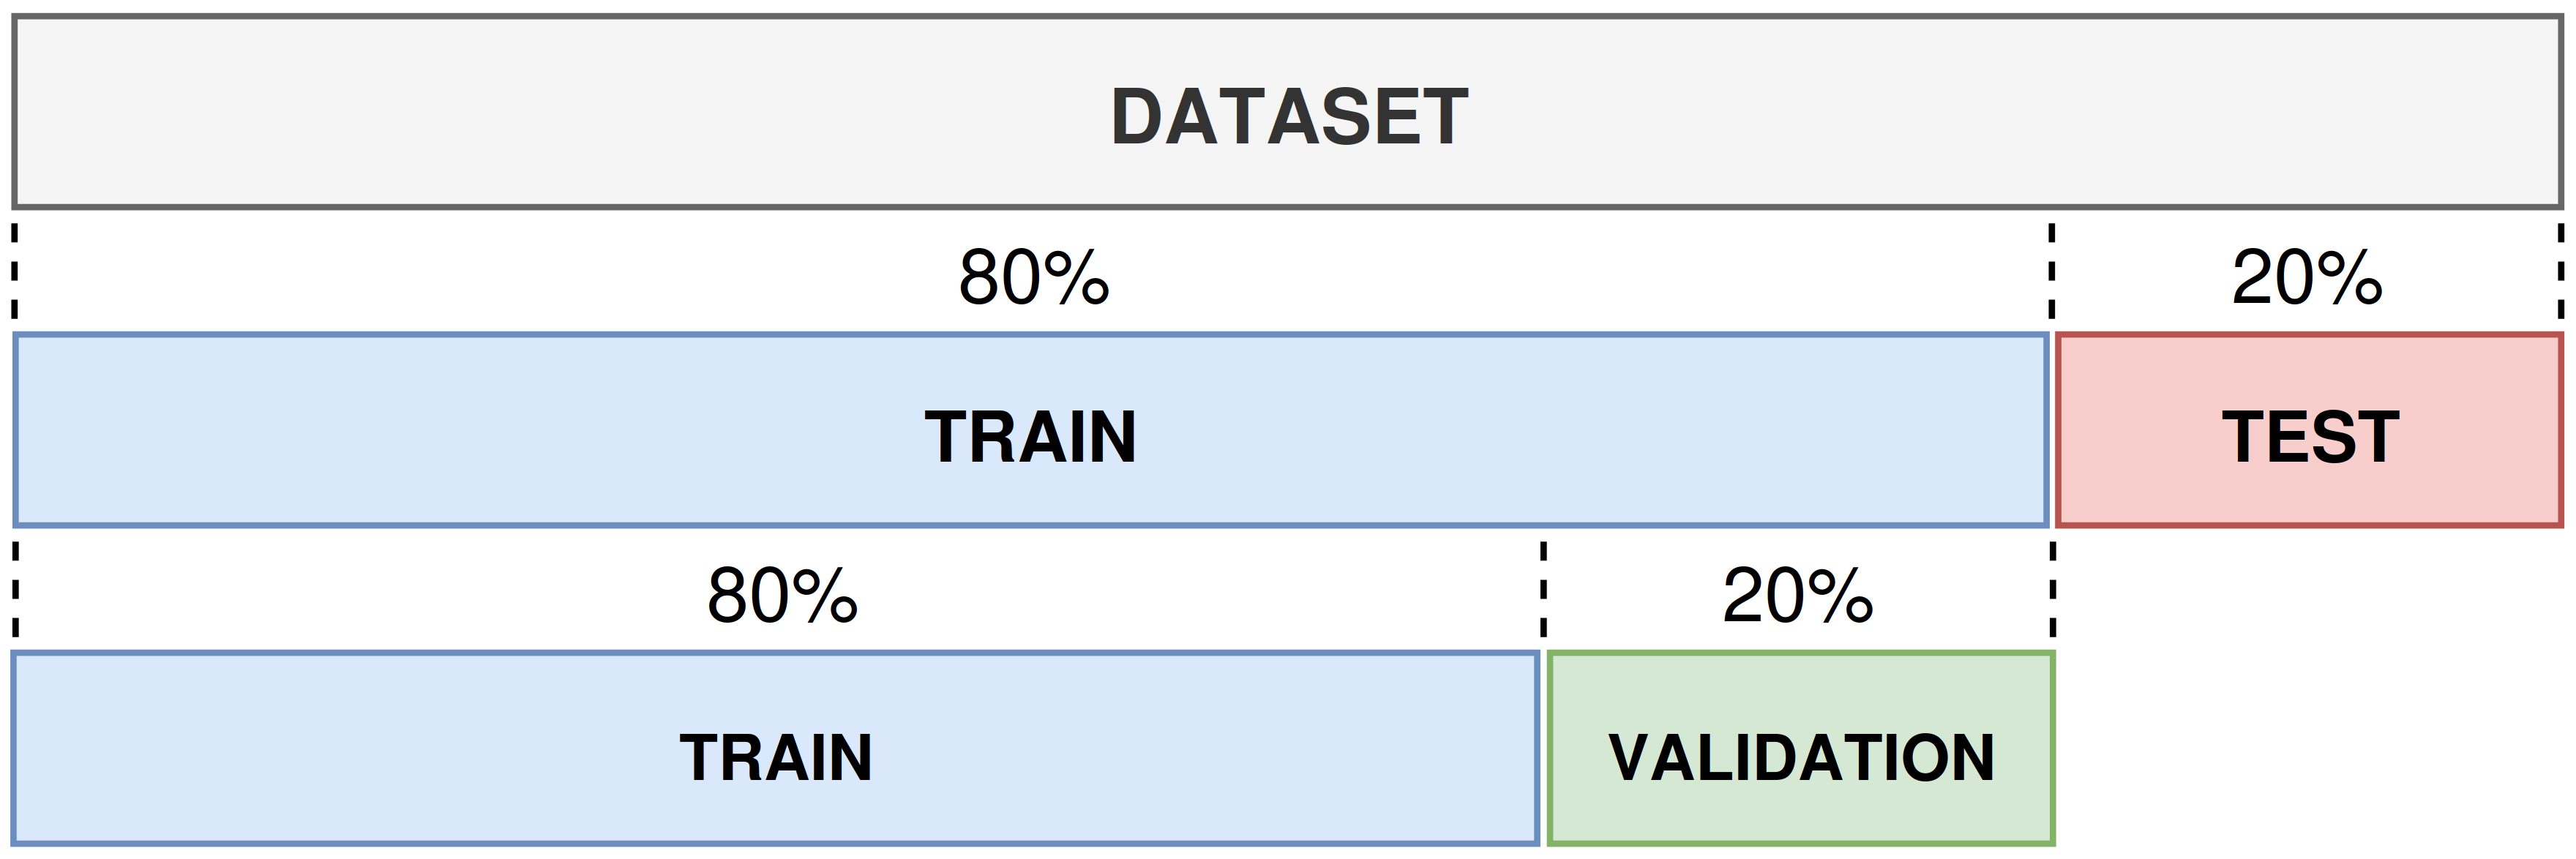
\includegraphics[width=0.8\textwidth]{capitulos/cap_04/imagenes/data_split_base.png}
    \caption[
        Diagrama de división del \textit{dataset} en \textit{train}, \textit{validation} y \textit{test}.
    ]{
        Diagrama de división del \textit{dataset} en \textit{train}, \textit{validation} y \textit{test}. 
        Elaboración propia.
    } 
    \label{fig:data_split_base}
\end{figure}

Sin embargo, al emplear métodos de calibración o predicción conformal, si usamos los mismos datos de 
entrenamiento para la calibriación, 
las probabilidades o intervalos de predicción tenderán a ser optimistas, pues el modelo ha sido entrenado
con esos datos \cite{niculescu2005}. Por tanto, para evitar el sobreajuste y garantizar validez estadística 
se requiere de un subconjunto de datos adicional: el \textbf{conjunto de calibración}. Yo he escogido el 
15\% de los ejemplos de entrenamiento para calibración, basándome en los resultados empíricos de 
\cite{sesia2020} (que recomienda entre un 10\% y 30\% de datos de entrenamiento dedicados a calibración), 
tal y como se muestra en la Figura \ref{fig:data_split_conformal}.

\begin{figure}[h]
    \centering
    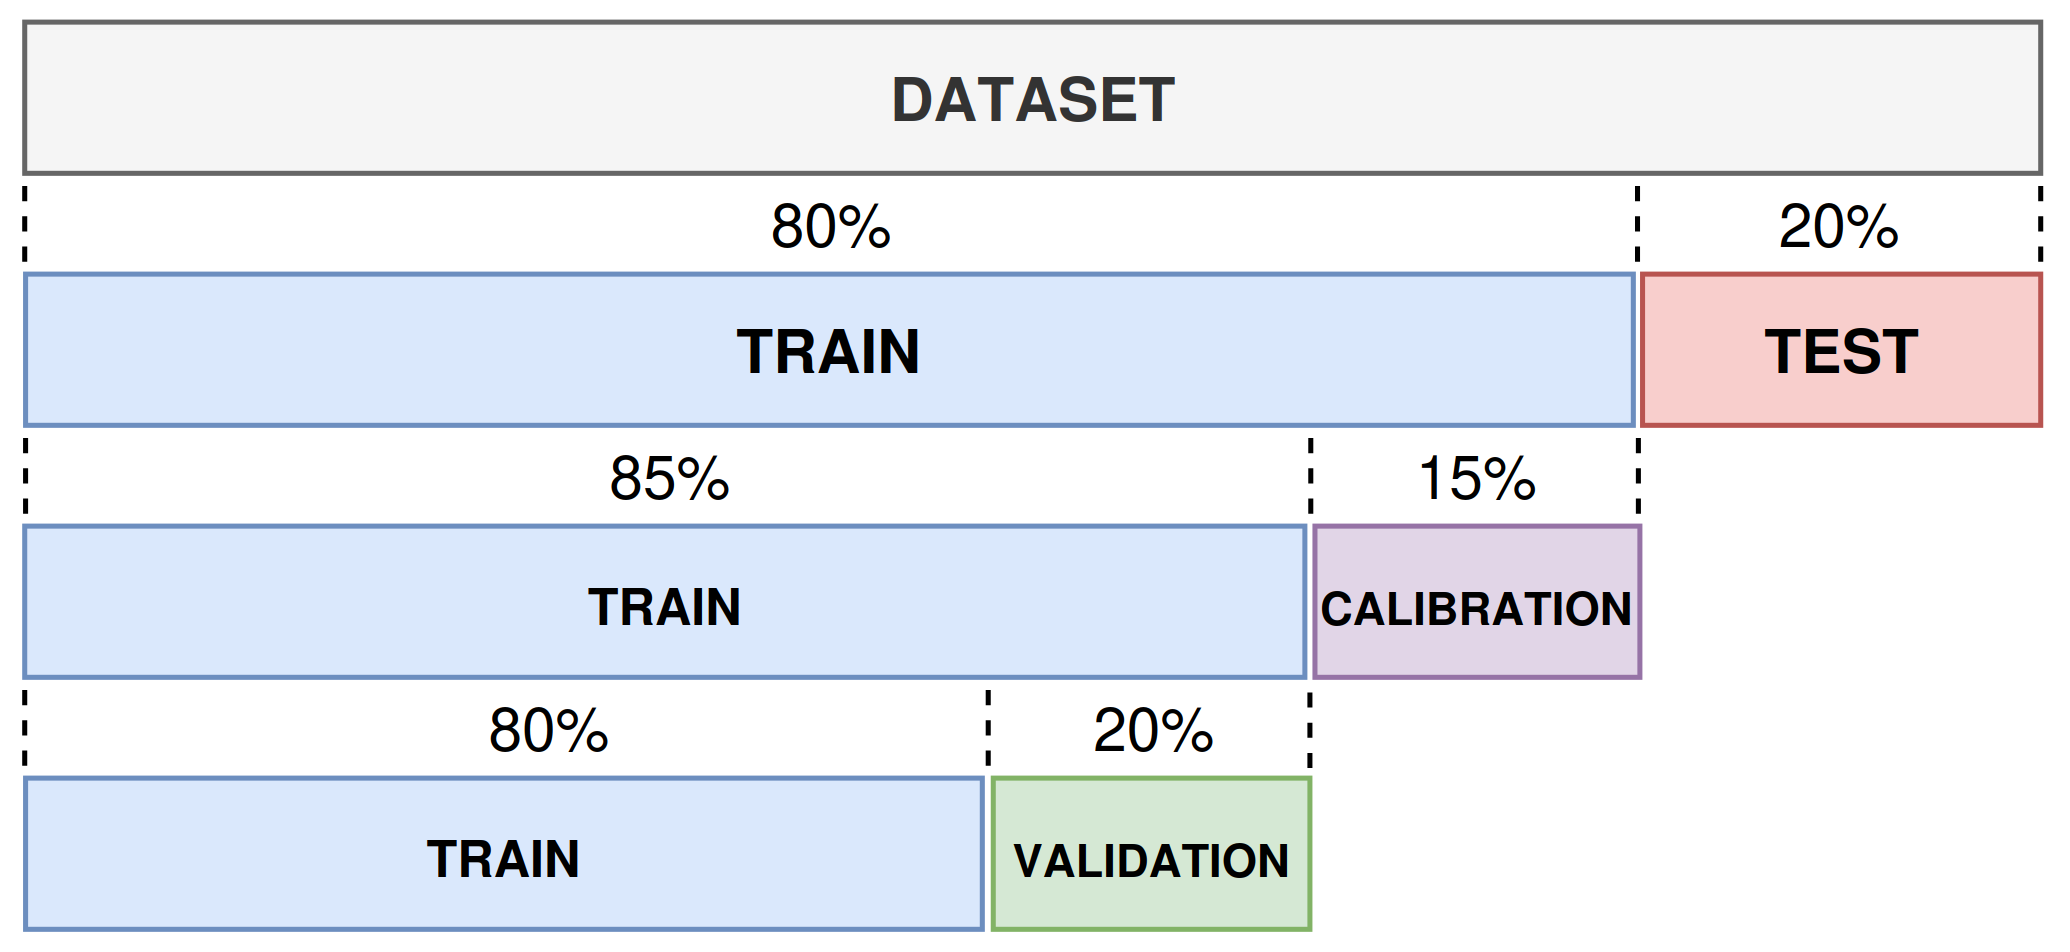
\includegraphics[width=0.8\textwidth]{capitulos/cap_04/imagenes/data_split_conformal.png}
    \caption[
        Diagrama de división del \textit{dataset} en \textit{train}, \textit{validation}, \textit{calibration} 
        y \textit{test}.
    ]{
        Diagrama de división del \textit{dataset} en \textit{train}, \textit{validation}, \textit{calibration}
        y \textit{test}. Elaboración propia.
    } 
    \label{fig:data_split_conformal}
\end{figure}

Para una comparativa más justa entre métodos que usan CP y los que no, se utilizará la siguiente estrategia: 
los métodos que no emplean Conformal Prediction (CP) seguirán el esquema tradicional de división de datos 
(entrenamiento, validación y test), mientras que los métodos basados en CP incorporarán además un conjunto 
de calibración independiente. Esta diferencia en el diseño experimental nos permitirá cuantificar cómo afecta 
a la capacidad predictiva de los modelos el hecho de reservar parte de los datos para el proceso de 
calibración.






% El objetivo del ML es establecer una hipótesis que se ajuste de forma óptima a los ejemplos futuros. Para 
% ello, suponemos que los ejemplos futuros mostrarán un comportamiento similar a los pasados. Bajo este 
% supuesto, el ajuste óptimo de un modelo es, por tanto, la hipótesis que minimiza la tasa de error del 
% problema \cite{rusell2021}. 

% Pero medir el error del modelo sobre los mismos datos empleados en el entrenamiento suele sesgar el resultado, 
% ya que el modelo puede estar sobreajustado (\textit{overfitting}) a los datos de entrenamiento, capturando no 
% solo el patrón subyacente, sino también el ruido o las peculiaridades específicas de ese conjunto de datos.
% Para evitar esto, es fundamental evaluar el modelo en un conjunto de datos de prueba independiente, que simule 
% cómo se comportaría con ejemplos futuros no vistos durante el entrenamiento. Por este motivo, es común dividir 
% los datos disponibles en dos conjuntos distintos: el \textbf{conjunto de entrenamiento (\textit{training 
% set})} y \textbf{conjunto test (\textit{test set})}.

% Aun así, incluso con esta división de conjuntos, puede persistir el riesgo de sobreajuste si se realizan 
% múltiples ajustes y selecciones de hiperparámetros basados en el rendimiento en el conjunto test.
% Esto se debe a que, indirectamente, el modelo podría estar ``aprendiendo'' características específicas del 
% conjunto de prueba, comprometiendo su capacidad de generalización. Para abordar este problema, se introduce 
% un tercer subconjunto: el \textbf{conjunto de validación}. Este conjunto se utiliza para evaluar y ajustar 
% los hiperparámetros del modelo durante el desarrollo, reservando el conjunto test únicamente para la 
% evaluación final.

% Además, técnicas como la \textbf{validación cruzada (\textit{cross-validation})} son ampliamente utilizadas 
% para maximizar el uso de los datos disponibles, especialmente en conjuntos pequeños. En lugar de una única 
% división entrenamiento-validación, este método:

% \begin{enumerate}
%     \item Divide los datos en $k$ particiones (\textit{folds}) (véase la Figura \ref{fig:CVDiagram}).
%     \item En cada iteración, usa $k-1$ particiones para entrenamiento y la restante para validación, rotando
%     sistemáticamente la partición de validación hasta que cada una de las $k$ particiones haya sido utilizada 
%     exactamente una vez como conjunto de validación. 
%     \item Promedia los resultados de todas las iteraciones para obtener una métrica robusta.
% \end{enumerate}

% El modelo final se entrena con todos los datos de entrenamiento (incluyendo los usados en validación durante 
% el ajuste). Si bien esta técnica proporciona estimaciones más confiables, su costo computacional es 
% significativo, ya que requiere entrenar el modelo $k+1$ veces ($k$ iteraciones de validación más el 
% entrenamiento final), lo que puede ser prohibitivo para modelos complejos, como redes neuronales profundas.

% \begin{figure}[h]
%     \centering
%     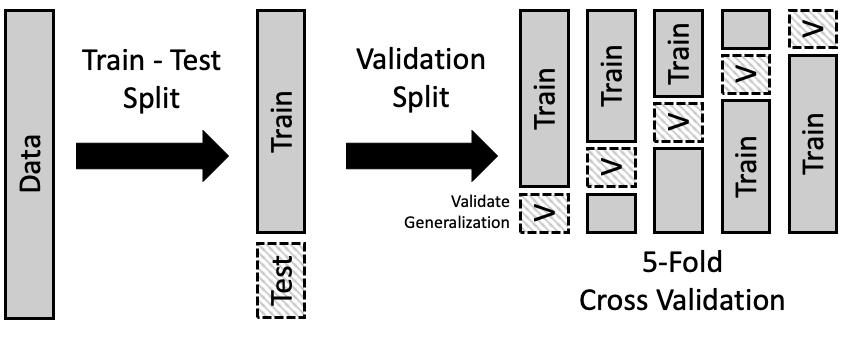
\includegraphics[width=0.95\textwidth]{capitulos/cap_05/imagenes/CVDiagram.png}
%     \caption{
%         Diagrama de división del dataset para la validación cruzada. 
%         Recuperado de \cite{lau2023crossvalidation}.
%     } 
%     \label{fig:CVDiagram}
% \end{figure}

% ------------------------------------------------------------------------------------------------------------
% ------------------------------------------------------------------------------------------------------------

\section{Entrenamiento del modelo}

\subsection{Preparación de los datos de entrenamiento}

Ya tenemos el conjunto de datos que se destina a esto. Se ha establecido un tamaño de \textit{batch} de 32, 
tras encontrar preeliminarmente un equilibrio entre regularización y buen ritmo de aprendizaje. 
Y también se ha realizado \textit{data augmentation} en el conjunto de entrenamiento, introduciendo 
transformaciones aleatorias en cada época para simular condiciones de posicionamiento del paciente y de la 
máquina e iluminación ligeramente variables: 
\begin{itemize}
    \item volteo horizontal en la mitad de las imágenes,
    \item rotación entre -3 y 3 grados,
    \item traslaciones de hasta el 2\%,
    \item escalado entre el 95 y 105\%, y
    \item cambios de brillo y contraste entre 80 y 120\%. 
\end{itemize}


\subsection{Adaptación de la red para la estimación de edad}

Como se venía anticipando en el anterior capítulo, cambiaremos la cabecera del modelo ResNeXt50 por otra 
para realizar la regresión. Sustituiremos la última capa del modelo por un \textit{adaptive average pooling}
---que se concatena con un \textit{sex embedding} de 8 dimensiones, en caso de utilizarse este metadato---
justo antes de la capa de \textit{flatten}, seguida por dos bloques que contienen una 
\textit{batch normalization}, una capa de \textit{dropout} y una capa FC, con una activación ReLU entre 
ambos bloques. La primera capa FC tiene 4.096 neuronas, la segunda 512, y finalmente una capa de salida 
de una sola neurona. 

\todo{Añadir un dibujo con el cambio de cabecera (AGOSTO)}

Los componentes clave del \textit{pipeline} de entrenamiento son:

\begin{itemize}
    \item Error cuadrático medio (\textit{mean squared error}, MSE) como función de pérdida en modelos de 
    predicción puntual y \textit{pinball} para modelos QR. 
    
    MSE es la función de pérdida por defecto para problemas de regresión, por muchas razones: los errores 
    siguen una distribución normal, lo que hace que minimizar el MSE equivalga a maximizar la verosimilitud 
    de los datos bajo este supuesto; penaliza los errores grandes más que proporcionalmente en comparación 
    con los pequeños, lo que ayuda a evitar predicciones extremadamente alejadas de los valores reales; y es 
    derivable en todo su dominio, ---además de que su derivada es lineal, lo que facilita el cálculo en la 
    retropropagación---, y convexa, lo que garantiza la existencia de un único mínimo global, facilitando la 
    convergencia en problemas lineales.
        
    \item Optimizador AdamW \cite{loshchilov2017}. Se ha escogido este optimizador dado que, por lo general,
    no requiere un ajuste exhaustivo de hiperparámetros para lograr buenos resultados. 
    
\end{itemize}

Para el entrenamiento de la nueva cabecera, se han congelado todas las capas de la arquitectura salvo las 
nuevas capas FC, de las cuales se han entrenado los pesos con \textit{learning rate} de 3e-2 y 
\textit{weight decay} 2e-4 durante dos épocas. 

Tras esto, se ha entrenado la red completa. Primero, se han descongelado todas las capas del modelo y se ha 
establecido \textit{learning rate} discriminativo por capas, siguiendo una escala exponencial desde 1.5e-4 en 
las capas más supeficiales hasta 1.5e-2 en las capas más profundas. 

Además, se ha usado el \textit{learning rate scheduler}, que modifica el \textit{learning rate} según una 
estrategia adaptativa. En concreto, se ha utilizado el método OneCycle \cite{smith2018}, que sigue una 
política cíclica de un solo ciclo, en la que el learning rate se incrementa progresivamente desde un valor 
inicial bajo hasta un valor máximo, para luego disminuir de forma suave hasta un valor final aún menor. Esta 
estrategia busca acelerar la convergencia durante las primeras etapas del entrenamiento y afinar los pesos en 
las etapas finales, mejorando el rendimiento general del modelo.

Se ha establecido un número de 30 épocas. 
Para evitar un posible sobreajuste del modelo, se ha hecho \textit{checkpointing} con los pesos
correspondientes a la época en la que se obtuvo la mejor puntuación en el conjunto de validación, permitiendo 
así conservar el estado del modelo con mayor capacidad de generalización (el que haya obtenido menor pérdida
en validación). Estos pesos se restauran al final del entrenamiento.

% ------------------------------------------------------------------------------------------------------------
% ------------------------------------------------------------------------------------------------------------

\section{Métricas}

\subsection{Métricas para regresión}

En nuestro problema de regresión emplearemos dos tipos de métricas con el objetivo de evaluar aspectos 
distintos del desempeño del modelo.

Por una parte, las métricas destinadas a las predicciones puntuales se basan fundamentalmente en medir el 
error entre el valor real ($y_i$) y el predicho ($\hat{y_i}$). Estas métricas nos permiten cuantificar 
directamente la discrepancia entre las estimaciones del modelo (estimación central en modelos de predicción
interválica) y la \textit{ground truth}. Las métricas que empleamos para estas predicciones son:

\begin{itemize}
    \item El \textbf{error absoluto medio (\textit{mean absolute error}, MAE)} mide el promedio de las 
    diferencias absolutas entre los valores reales ($Y_i$) y los valores predichos ($\hat{Y_i}$) por el 
    modelo.

    $$
    MAE = \frac{1}{n} \sum_{i=1}^n{|y_i - \hat{y_i}|} \in [0, \infty)
    $$

    donde $n$ es el número de ejemplos/instancias con las que se cuenta en los datos a evaluar.

    La interpretación más inmediata de esta métrica es que representa cuánto se desvía en promedio la 
    predicción del valor real sin considerar la dirección del error (positivo o negativo) y, por tanto, cuanto 
    más se acerque a cero el valor, mejor es el ajuste del modelo.

    \item El \textbf{error cuadrático medio (\textit{mean squared error}, MSE)} mide el promedio de los 
    errores al cuadrado entre valores reales ($Y_i$) y los valores predichos ($\hat{Y_i}$) por el modelo.
    
    $$
    MSE = \frac{1}{n} \sum_{i=1}^n{(y_i - \hat{y_i})^2} \in [0, \infty)
    $$

    Al igual que el MAE, cuantifica qué tan cerca están las predicciones de los valores reales, pero penaliza
    más los errores grandes, y es más sensible por tanto a valores atípicos.

\end{itemize}


Por otra parte, las métricas aplicadas a las predicciones interválicas examinan tanto la capacidad del modelo 
para abarcar el valor real dentro del intervalo predicho ---conocida como 
\textbf{cobertura (\textit{coverage})}--- como la \textbf{amplitud} del mismo, que es el ancho del rango de valores 
del intervalo de predicción. 
Generalmente, existe un equilibrio entre ambos aspectos: al aumentar la amplitud, es más probable que el 
intervalo contenga el valor real, pero esto disminuye la precisión y utilidad práctica de la predicción.
Veamos las métricas para este tipo de predicciones: 

\begin{itemize}
    \item La \textbf{cobertura empírica (\textit{empirical coverage}, EC)} cuantifica la proporción de valores
    reales dentro de los intervalos de predicción obtenidos. 
    
    $$
    EC = \frac{1}{n} 
        \sum_{i=1}^n{ \mathbb{I} \left[ y_{{lower}_i} \le y_i \le y_{{upper}_i} \right] } 
            \in \left[0, 1\right]
    $$

    Cuanto mayor sea el valor, mejor cobertura ofrece el modelo, si bien coberturas altas suelen conllevar 
    intervalos excesivamente amplios, lo que reduce su utilidad práctica. Es por ello que, empleando métodos
    de CP, tiene más sentido que el objetivo sea acercarse lo máximo posible a la cobertura marginal 
    nominal ($1-\alpha$), garantizando así intervalos de predicción que equilibren precisión y fiabilidad sin
    ser inneceseriamente conservadores. 
    
    \item El \textbf{tamaño de intevalo medio (\textit{mean inteval width}, MIW)} mide qué tan amplios son en 
    promedio los intervalos predichos.
    
    $$
    MIW = \frac{1}{n} \sum_{i=1}^n{ \left( y_{{upper}_i} - y_{{lower}_i} \right) } \in (0, +\infty)
    $$
    
    Se desea matener este valor lo más pequeño posible, dado un nivel de cobertura adecuado. Valores altos
    indican intervalos anchos y, por tanto, poco útiles para la toma de decisiones. 


    % \item La \textbf{\textit{interval score} (IS)} \cite{gneiting2007} trata de unificar en una sola métrica
    % el \textit{trade-off} cobertura vs. ancho. Su expresión es la siguiente:

    % $$
    % IS = \frac{1}{n} \sum_{i=1}^n{
    %         \left(         
    %             (u_i-l_i) 
    %             + \frac{2}{\alpha} \left( l_i-y_i \right) \mathbb{I}\left[ y_i<l_i \right] 
    %             + \frac{2}{\alpha}  \left( y_i-u_i \right) \mathbb{I}\left[ y_i>u_i \right]
    %         \right)
    %     }
    % $$

    % El primer término ($u_i-l_i$) penaliza la anchura del intervalo de predicción, incentivando intervalos 
    % más precisos y estrechos.
    
    % El segundo y tercer término penalizan los casos en que el valor real cae fuera del intervalo, con una 
    % penalización proporcional a la distancia entre el valor verdadero y el borde del intervalo. Además, esta 
    % penalización se ajusta por el nivel de significancia $\alpha$, de modo que a niveles de confianza más 
    % altos (es decir, $\alpha$ más pequeños), las penalizaciones por valores fuera del intervalo son más 
    % severas.

\end{itemize}

Y, finalmente, también añadiremos elementos visuales para valorar el desempeño de la CP:

\begin{itemize}

    \item \textbf{Gráfica de dispersión EC - MIW}: Este gráfico permite visualizar el compromiso entre 
    cobertura lograda y tamaño del intervalo. Un buen modelo debería situarse cerca del nivel de confianza 
    objetivo con intervalos lo más cortos posible.
    
    \item \textbf{Gráficas de densidad de tamaños de intervalos}: Esto nos permitirá analizar la distribución 
    de las longitudes de los intervalos predichos. Una concentración alrededor de valores bajos indica 
    intervalos más informativos, mientras que una distribución amplia o con colas largas puede revelar
    incertidumbre elevada en ciertos casos. Esta visualización nos será útil para aquellas técnicas que 
    ofrecen intervalos predictivos adaptativos. 

\end{itemize}

% ------------------------------------------------------------------------------------------------------------

\subsection{Métricas para clasificación}

\todo{Por completar (JULIO)}

% ------------------------------------------------------------------------------------------------------------
% ------------------------------------------------------------------------------------------------------------

\section{Ajuste de hiperparámetros de predicción conformal}

No hay ninguna técnica (por ahora) que requiera ajuste de hiperparámetros. 

% ------------------------------------------------------------------------------------------------------------
% ------------------------------------------------------------------------------------------------------------

\section{Resultados}





\begin{figure}[h]
    \centering
    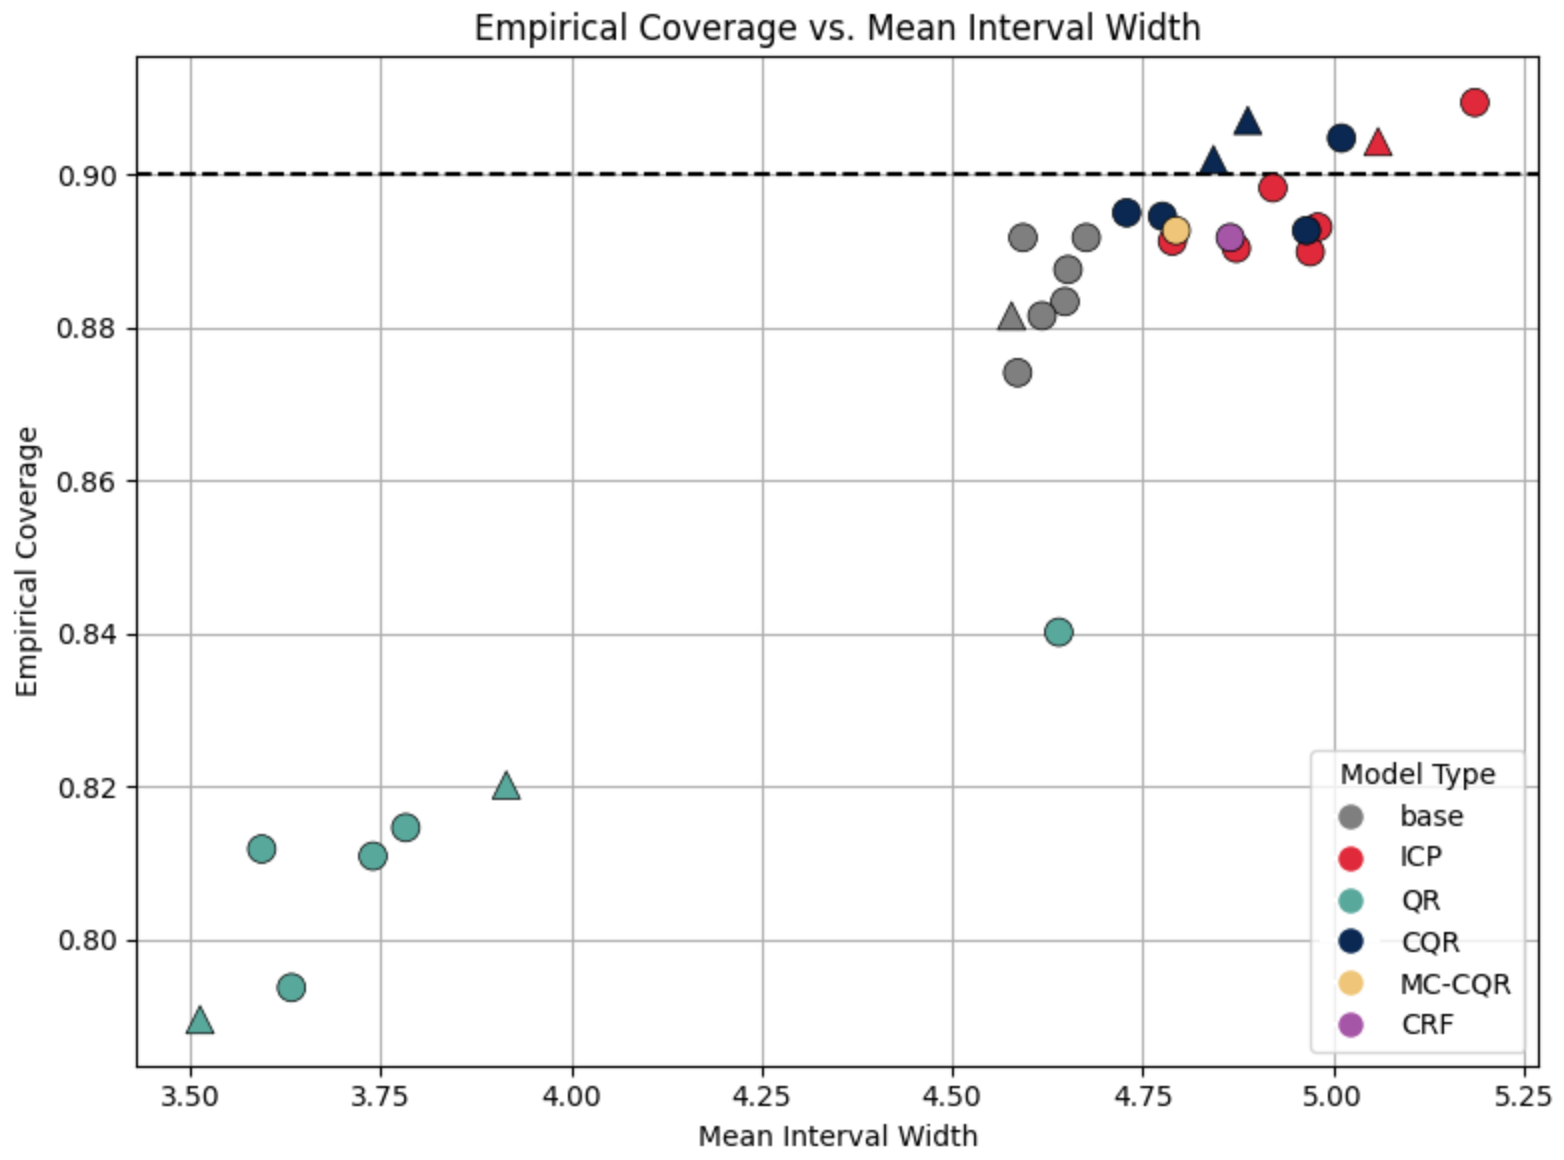
\includegraphics[width=\textwidth]{capitulos/cap_05/imagenes/EC-MIW.png}
    \caption[
        Gráfica de dispersión EC-MIW
    ]{
        Gráfica de dispersión EC-MIW. Triángulo = con sex embedding. 
    }
    \label{fig:ec-miw}
\end{figure}


\begin{figure}[h]
    \centering
    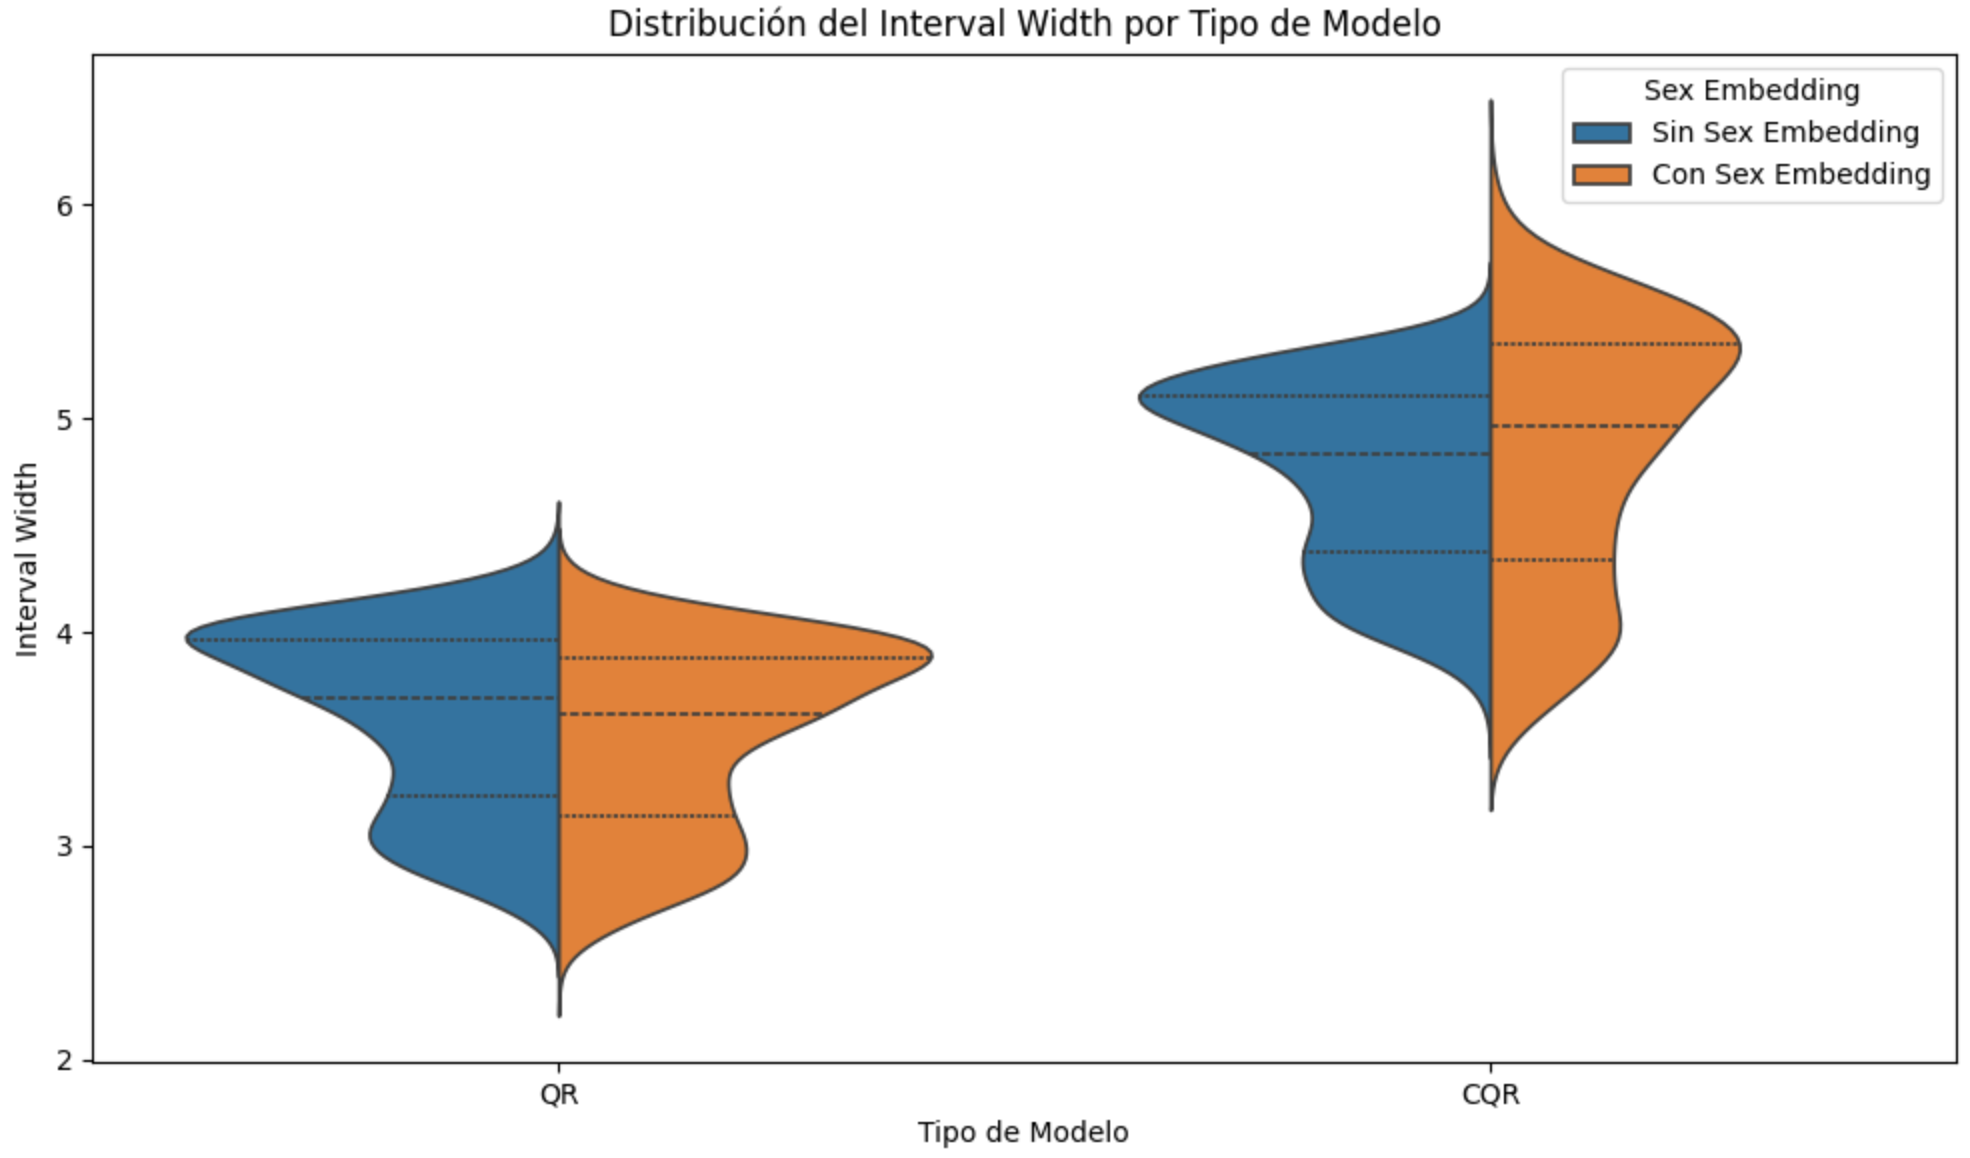
\includegraphics[width=\textwidth]{capitulos/cap_05/imagenes/violin_interval_width.png}
    \caption[
        Gráfica de violin de tamaños de intervalos
    ]{
        Gráfica de violin de tamaños de intervalos.
        Con estas diferencias entre problema con sex embedding y sin sex embedding, no sé si merece la pena
        esta comparación. Mi idea era que con sex embedding se reduciría la incertidumbre del problema y los 
        intervalos quedarías más ajustados, pero el rendimiento del modelo no mejora, y tampoco lo hacen por 
        consiguiente los intervalos de la CP. 
    }
    \label{fig:violin_interval_width}
\end{figure}


\begin{figure}[h]
    \centering
    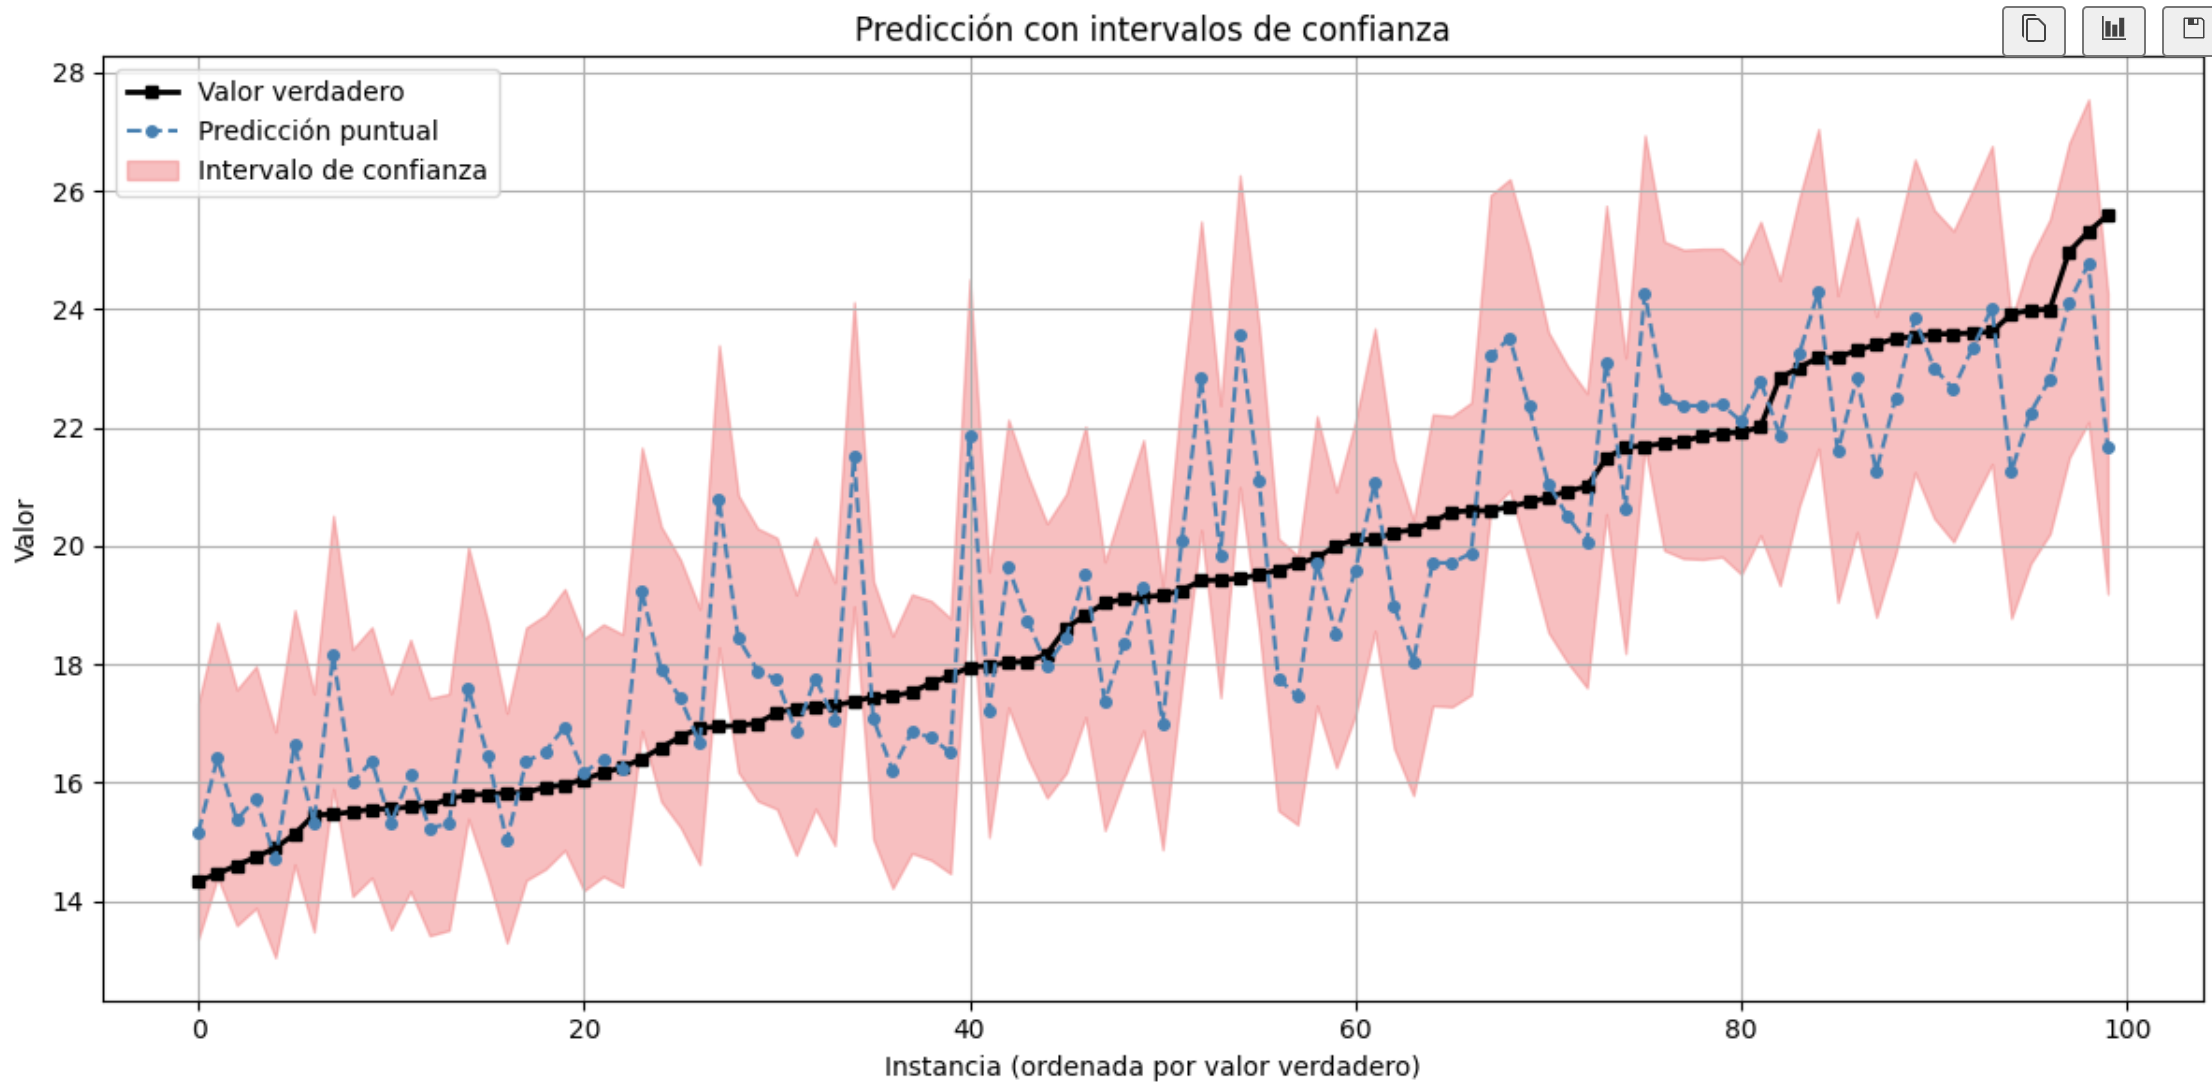
\includegraphics[width=\textwidth]{capitulos/cap_05/imagenes/conformal_prediction_sorted_by_true.png}
    \caption[
        Gráfica de líneas con predicción central e intervalo predictivo ordenado por valor real
    ]{
        Gráfica de líneas con predicción central e intervalo predictivo ordenado por valor real
    }
    \label{fig:conformal_prediction_sorted_by_true}
\end{figure}

\todo{Mejorar el diseño y legibilidad de todas las gráficas (JULIO)}


% ------------------------------------------------------------------------------------------------------------
% ------------------------------------------------------------------------------------------------------------


